\documentclass[english]{article}
\usepackage{geometry}
\usepackage{hyperref}
\usepackage{inputenc}
\geometry{verbose,tmargin=3.5cm,bmargin=4cm,lmargin=3.8cm,rmargin=3.8cm}
\usepackage[backend=biber,style=ieee]{biblatex}
\addbibresource{sources.bib}
\makeatletter
\usepackage{url}
\usepackage{graphicx}
\usepackage{caption}
\usepackage{wrapfig}
\usepackage{subcaption}
\makeatother
\usepackage{babel}

\begin{document}
	
	\title{Multi-Agent Path Finding with Matching using Increasing Cost Tree Search}
	
	\author{Thom van der Woude\and Jesse Mulderij\and Mathijs de Weerdt}
	\date{}
	
	\maketitle
	
	\begin{abstract}
		Both the assignment problem and the multi-agent pathfinding problem are common problems in fields such as robotics and transportation. The joint problem of finding matchings inducing an optimal non-conflicting routing of agents to their goals is something that has not been studied much. Few methods exist today that solve it although the problems do appear together in real-world problems, such as in the Train Unit Shunting and Servicing problem. In this work, a novel method based on the Increasing Cost Tree Search algorithm for multi-agent pathfinding is presented that can optimally solve this joint problem.
	\end{abstract}
	
	\section{Introduction}
	The Dutch Railways (NS) company\footnote{\url{https://www.ns.nl/}} needs to clean and service their fleet of trains during the night in shunting yards so that they can properly bring passengers from A to B during the day. 
	The problem of scheduling the trains and personnel to achieve this is called the Train Unit Shunting and Servicing (TUSS) problem \cite{mulderij2020}. 
	It is an NP-hard problem with many different subproblems in addition to the basic train unit routing, such as the timetabling of personnel and coupling and decoupling of train units entering and leaving the yard. % introduce heuristics here.
	
	As was shown by Geiger et al.\cite{geiger2018}, in practical scenarios, only heuristic methods can solve TUSS instances. 
	Such methods are suboptimal and heuristic solutions to instances defined for a set shunting yard can be said to characterise a lower bound on the capacity of the shunting yard, as each solution cost gives a (loose) upper-bound for the optimal solution cost. 
	The railway company, however, is interested in learning tight upper bounds for the capacity of existing shunting yards to inform decisions about matters like infrastructure expansion. 
	Mulderij et al. \cite{mulderij2020} propose the multi-agent pathfinding (MAPF) problem \cite{stern2019} extended with a matching subproblem (hereafter MAPFM) as a suitable relaxation for finding such upper-bounds using an approach analogous to that outlined above.
	For this to succeed, a way to optimally solve MAPFM instances is needed.

	Comparatively, little research has been done on MAPFM and solving MAPFM optimally.
	The Conflict-Based Min-Cost-Flow (CBM) algorithm by Ma and Koenig \cite{ma2016} is one of the few existing approaches to optimally solve this more general problem along with the somewhat similar one described in \cite{henkel2019}.
	Ma and Koenig's method builds upon the conflict-based search method and in particular on the Meta-Agent variation thereof also discussed in \cite{sharon2015} as a high-level search framework, while exploiting the connection between MAPF problems and max-flow problems (as discussed in \cite{yu2013}) in the low-level search. It should be noted that this method minimizes the makespan and not the sum of individual costs which is the objective used in the TUSS relaxation, meaning that non-trivial modifications to CMB are needed in order to minimize SIC.
	The successful application of CBS to solving MAPFM begs the question: can alternative MAPF algorithms such as Increasing Cost Tree Search (ICTS) \cite{sharon2011} or M* \cite{wagner2011} also serve as the basis for a MAPFM solver?
		
	\begin{wrapfigure}{R}{.25\textwidth}
		\begin{minipage}{\linewidth}
			\centering\captionsetup[subfigure]{justification=centering}
			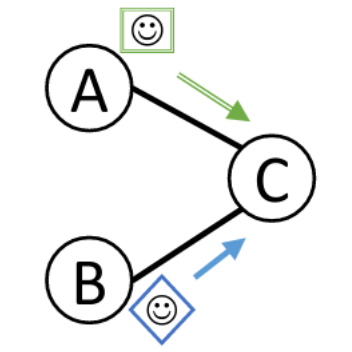
\includegraphics[width=\linewidth]{img/vertex-conflict}
			\subcaption{Vertex conflict}
			\label{fig:conflictsa}\par\vfill
			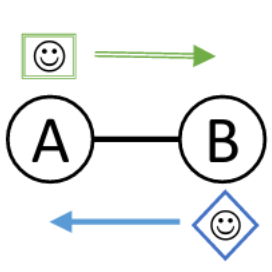
\includegraphics[width=0.75\linewidth]{img/edge-conflict}
			\subcaption{Swapping conflict}
			\label{fig:conflictsb}
		\end{minipage}
		\caption{The two types of conflict (from Fig. 1 in \cite{stern2019})}\label{fig:conflicts}
	\end{wrapfigure}
	This work is the outcome of a search for an efficient algorithm for optimally solving MAPFM derived from ICTS as an alternative to the approach outlined above\footnote{To the knowledge of the author, to date, no such algorithm is described in the literature}. ICTS, in short, is a two-level approach to MAPF with a top-level breadth-first traversal of an Increasing Cost Tree (ICT) representing combinations of per-agent path costs and a bottom-level evaluation of ICT nodes using multi-valued decision diagrams (MDDS). These MDDS represent per agent all possible paths to the goal of a set length. In the context of a research project in which multiple such 
	MAPF algorithms were taken as starting points for MAPFM algorithms within a group, the novel ICTS-based algorithm is compared to these algorithms on a set of benchmarks similar to those described in \cite{stern2019}. In addition, it is analysed in terms of complexity and compared to both an enumerative approach that solves all matchings using regular ICTS and the algorithm described in \cite{ma2016}. Lastly, completeness of the algorithm is considered as this is a key property in the context of MAPFM as a TUSS relaxation. Regarding the relevance of this work, it should be noted that besides TUSS, there are other applications such as planning warehouse robots \cite{wurman2007} that also could benefit from novel algorithms for MAPFM.

	\section{Multi-agent pathfinding with matching} % Problem description
	The MAPFM problem is an extension of MAPF, a well-studied problem. Formally, a MAPF instance can be described as follows. Let $G = (V,E)$ be an undirected connected graph, with each $v\in V$ representing an obstacle-free tile on a 4-connected grid and each $e = (u,v)\in E$ representing a legal uniform-cost move between two such tiles. Let there be $k$ agents $a_1,\ldots,a_k$ with respective starting locations $s_1,\ldots,s_k$ and goals $g_1,\ldots,g_k$. For each agent $a_i$, a path $\pi_i$ from $s_i$ to $g_i$ is to be found such that all agents paths $\pi_i$ taken together are non-conflicting and therefore are a solution. In this work, non-conflicting means, in the conflict-terminology of \cite{stern2019}, that there are no vertex conflicts (and thus no edge conflicts) and no swapping conflicts, as shown in Figure \ref{fig:conflicts}. Letting $\pi_i^t$ denote the $t$'th node of path $\pi_i$, this means that for $i\neq j$, for all $t$, $\pi_i^t\neq \pi_j^t$ and $(\pi_i^t \neq \pi_j^{t + 1})\lor(\pi_i^{t+1} \neq \pi_j^t)$. Given a solution $(\pi_1,\ldots,\pi_k)$, a vector of per-agent costs $(c_1,\ldots,c_k)$ can be found. For $\pi_i$, $c_i$ is defined as the time at which $a_i$ reaches $g_i$ for the last time and remains there, meaning that for $t \geq c_i$, $\pi_i^{t} = g_i$. One property of $c_i$ is that $c_i \geq c^*_i$ where $c^*_i$ is defined as the cost of $\pi^*_i$, the shortest path from $s_i$ to $g_i$. There are two common objectives in MAPF:
	\begin{itemize}
		\item The makespan: $\max_{i} c_i$
		\item The sum of individual costs (SIC): $\sum_i c_i$
	\end{itemize}
	In this work, following the definition of the TUSS relaxation in \cite{mulderij2020}, an optimal solution is defined as having minimal SIC. Note that $\sum_i c_i \geq \sum_i c^*_i$
	\subsection{Increasing Cost Tree Search}
	In the above, given a combination of paths $(\pi_1,\ldots,\pi_k)$, a vector of costs is found from which the SIC is derived. This is a surjective mapping: many cost vectors $(c'_1,\ldots,c'_k)$ might add up to the same SIC as $(c_1,\ldots,c_k)$ and for a given agent $a_i$, there might be many equivalent paths $\pi'_i$ to the goal with cost $c_i$. On uniform-cost 4-grids in particular, there are often many equivalent and symmetrical solutions\cite{harabor2010} (see Figure \ref{fig:symmetries}), which is why in single-agent pathfinding, symmetry-breaking methods like Jump Point Search\cite{harabor2011} are used to speed up search. In multi-agent pathfinding, having multiple paths per agent of the same cost can, in contrast, be a boon: it means that there are potentially more non-conflicting ways to combine paths of different agents.
	\begin{figure}[t]
		\centering
		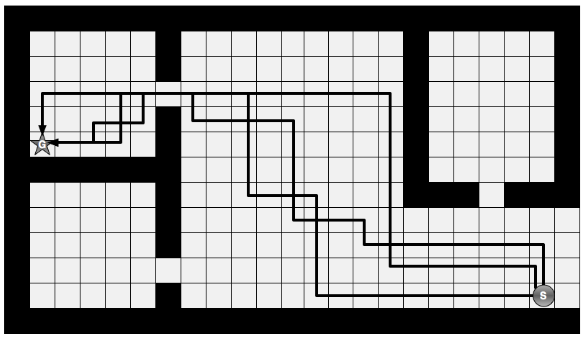
\includegraphics[width=0.4\linewidth]{img/symmetries}
		\caption{Symmetric paths on a 4-connected grid\cite{harabor2010}}
		\label{fig:symmetries}
	\end{figure}

	In Increasing Cost Tree Search\cite{sharon2011}, the above two-step mapping from path combination to cost vector and from cost vector to SIC is reversed in order to search for a solution with minimal SIC. This is done by searching for cost vectors corresponding to increasing SIC on the top level and searching for non-conflicting path combinations (solutions) for each cost vector on the bottom level. 
	
	\subsubsection{Top-level search}
	 In the top-level search, all possible cost vectors for a given SIC are evaluated by searching an Increasing Cost Tree as depicted in \ref{fig:ict}, starting from $C_{root} = \sum_i c^*_i$ corresponding to a single root cost vector $(c^*_1,c^*_2,\ldots,c^*_k)$. This root has $k$ children $(c^*_1 + 1,c^*_2,\ldots,c^*_k),(c^*_1,c^*_2 + 1,\ldots,c^*_k),\ldots,(c^*_1,c^*_2,\ldots,c^*_k + 1)$ all of cost $C = C_{root} + 1$. Searching this ICT breadth-first corresponds to evaluating all possible cost vectors corresponding to increasing cost $C$ starting with $C_{root}$. The number of cost vectors evaluated when searching up to a depth of $\Delta$ with vectors cost of $C_{root} + \Delta$ is $\mathcal{O}(k^\Delta)$. Node evaluation is done by a low-level search that searches for a solution $(\pi_1,\ldots,\pi_k)$ corresponding to the node costs $(c_1,\ldots,c_k)$.
		
	\begin{figure}[t]
		\centering
		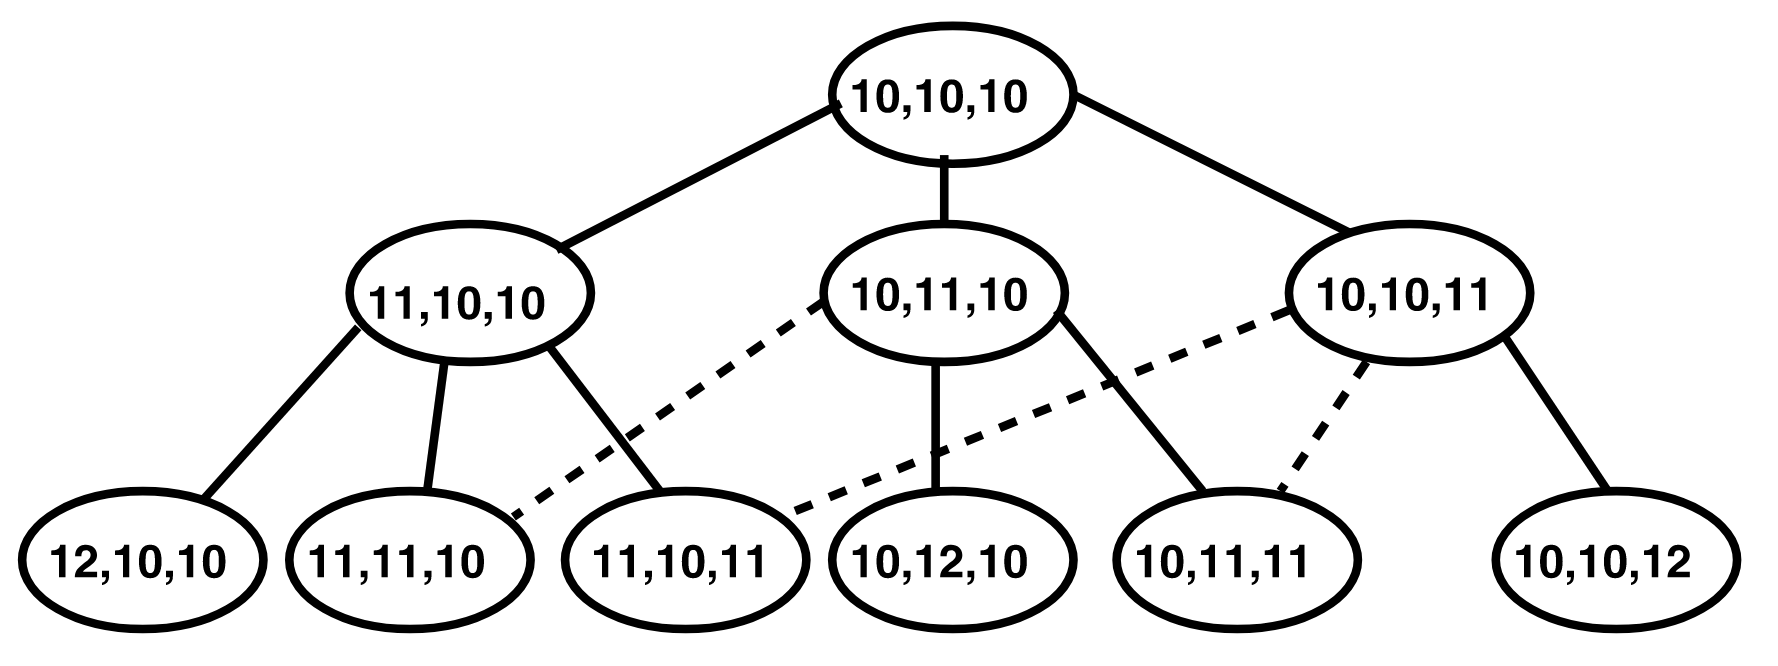
\includegraphics[width=0.7\linewidth]{img/ict}
		\caption{Increasing Cost Tree for three agents (Fig 4. in \cite{sharon2011})}
		\label{fig:ict}
	\end{figure}
	\subsubsection{Bottom-level search}
	Explicitly generating all paths of a set cost to the goal for each agent is expensive: the number of paths is exponential in the target cost. As the space of all path combinations for $k$ agents have to be searched, a more efficient method is required. This is why in the low-level search of ICTS, multi-valued decision diagrams (MDDS) are used to compactly represent all paths per agent and facilitate efficient search of the $k$-agent space of path combinations.
	
	Figure \ref{fig:symmetries} only shows a few possible paths of the same cost to the goal
	Evaluating a node in the above means performing a low-level search that searches the space of all combinations of paths $(\pi_1,\ldots,\pi_k)$ that correspond to the node costs $(c_1,\ldots,c_k)$.

	
	
	 the mapping from SIC to possible cost vectors, and from cost vectors to possible path combinations is reversed. 
	
	
	
	
	
	
	, w y might map to the same vector of costs and still more might yield the same SIC. 
	
	In an abstract sense, Increasing Cost Tree Search algorithm for MAPF \cite{sharon2011} can be thought of as exhaustively reversing this mapping.

	 

	
	
	Let there be $K$ teams $t_1,\ldots, t_K$, where $t_i$ consists of $k_i$ agents with start positions $s_1^i,\ldots,s_{k_i}^i$ together with an equal number of team goals $g_1^i,\ldots,g_{k_i}^i$. 
	
	

	Within each team $t_i$, agent $a_j^i$ are to be \textit{matched} to a unique goal $g_k^i$, so that exactly one agent is assigned to each goal within team $i$; once all agents are matched to goals, for each agent $a_j^i$ matched to $g_k^i$, a path from $s_j^i$ to $g_k^i$ is to be found such that all agents paths taken together are non-conflicting and therefore make up a solution \cite{ma2016}. In this work, non-conflicting means, in the conflict-terminology of 
	\paragraph{Old}
	MAPFM is the problem of finding agent-goal matchings that induce a non-conflicting routing of agents to their goals. Each matching corresponds to a MAPF instance, so each feasible matching has an optimal solution, i.e. a solution with a minimal Sum of Individual Costs (SIC). In approaching MAPFM as a TUSS relaxation to find upper-bounds for instances, optimal MAPFM solutions are the most interesting as they can characterise such upper-bounds. Furthermore, defining optimality as minimal SIC corresponds more closely to TUSS objective functions such as personnel cost than the other common MAPF objective, minimal makespan. Optimally solving MAPFM is equivalent to finding a feasible matching such that there is no other matching for which the corresponding MAPF instance has a lower optimal SIC. This motivates the joint nature of MAPFM: some matchings might be infeasible and others may have sub-optimal SIC costs, so especially in larger instances where there may be thousands of matchings, it is preferable to integrate the generation of matchings with the search for non-conflicting path-combinations to avoid having to exhaustively process all matchings. In this work, both integrated approaches and exhaustive methods using ICTS are considered.
	
	\subsection{Formulation}
	Formally, a MAPFM instance can be described as follows. Let $G = (V,E)$ be an undirected connected graph, with each $v\in V$ representing an obstacle-free tile on a 4-grid and each $e = (u,v)\in E$ representing a legal uniform-cost move between two such tiles. Let there be $K$ teams $t_1,\ldots, t_K$, where $t_i$ consists of $k_i$ agents with start positions $s_1^i,\ldots,s_{k_i}^i$ together with an equal number of team goals $g_1^i,\ldots,g_{k_i}^i$. 
	
	Within each team $t_i$, agent $a_j^i$ are to be \textit{matched} to a unique goal $g_k^i$, so that exactly one agent is assigned to each goal within team $i$; once all agents are matched to goals, for each agent $a_j^i$ matched to $g_k^i$, a path from $s_j^i$ to $g_k^i$ is to be found such that all agents paths taken together are non-conflicting and therefore make up a solution \cite{ma2016}. In this work, non-conflicting means, in the conflict-terminology of \cite{stern2019}, that there are no vertex conflicts (and thus no edge conflicts) and no swapping conflicts. Practically, this means that no two agents may be at $v\in V$ at the same timestep and that if agents $i,j$ are at locations $u,v$ respectively at timestep $t$, they may not be at locations $v,u$ at timestep $t+1$. 
	\section{Matching in ICTS} % Your contribution
	Two classes of algorithms were found for solving MAPFM optimally using ICTS-based methods. exhaustively enumerating MAPF instances corresponding to matchings solving these using a variant of regular ICTS, and modifying the increasing cost tree search itself to accomodate for the matching extension. In the following, both 
	
	
	
	Increasing Cost Tree Search with Matching (ICTS-m) generalizes ICTS to optimally solve MAPFM instances. Few changes to ICTS were necessary to accomodate for matching in this increasing cost tree scheme. Specifically, the ICT root generation and the MDD generation had to be changed. In regular ICTS, given a MAPF instance with agents $a_1,\ldots,a_k$ with goals $g_1,\ldots,g_k$ starting at locations $s_1,\ldots,s_k$, the root is given by the cost $c_i$ for each agent $a_i$ of the shortest path from $s_i$ to $g_i$, i.e. without taking conflicts into account. Any optimal pathfinding algorithm can be used for this. The root of the ICT then is the vector $(c_1,c_2,\ldots,c_k)$ with $k$ children $(c_1 + 1, c_2,\ldots,c_k), (c_1, c_2 + 1,\ldots,c_k),\ldots,(c_1, c_2,\ldots,c_k + 1)$ so that each component of the parent is incremented by 1 in exactly one child. This child-generation rule holds for all ICT nodes. 
	
	As described in \cite{sharon2011}, given $a_i$, generating all paths $(s_i,g_i)$ of a certain target cost $c_i$ can be accomplished by a breadth-first search on the $c_i$-steps time-expanded graph. Storing the resulting paths in an MDD, which has at most $|V|$ nodes at each timestep or depth, avoids the cost of storing all paths explicitly and also facilitates the efficient search of the $k$-agent space of path combinations.
	\subsection{Root generation for matching}
	Given a team $t_i$ of size $k_i$, for any agent $a_j^i$ there are $k_i$ costs $c_j(1),c_j(2),\ldots,c_j(k_i)$ for shortest paths from $s_j^i$ to each goal $g_k^i$. Making no assumptions about what goals other agents in $t_i$ are assigned to, it could be that in the optimal solution $a_j^i$ is assigned to a goal $g_{m}^i$ with cost $c_j(m)$ such that $c_j(m) = \min_{n\in\{0,\ldots,k_i\}} c_j(n)$. Therefore, to guarantee optimality, this minimal cost to any matching goal has to take the place of the shortest path cost from the original ICTS root. The resulting root is equivalent in the case that all teams are singleton. Intuitively, the sum of individual costs of this root is highly optimistic. Often, agents will not move to their closest matching goal in an optimal solution, even without considering conflicts.
	
	\subsection{MDD generation for matching}
	In MDD generation, each agent also has to consider not one goal but all matching goals. By following a BFS-based approach, with all team goals being goals in the search and in turn endpoints from which, using the time-expanded graph, the MDD was generated that is used in the low-level search, agent MDDs can be made to represent all possible paths of a set length to any matching goal. Once again, if all teams are singleton, the MDDs generated using this goal-set approach are the same as in regular ICTS.
	
	\subsection{Properties of ICTS-m}
	<insert proof>
	\section{Experimental results}
	\section{Responsible Research}
	In experiments used to compare the different MAPFM algorithms within the peer group, care was taken to make the comparison fair: all algorithms are implemented in Python 3 and run on the same system: a server with a 12-core Intel Xeon E5-2683 with 8Gb of RAM dedicated to running experiments for this project. Still, some implementations might be more optimized than others so this might be a factor in performance characteristics and in particular in relative performance differences.
	
	The implementation of the ICTS-based algorithms described in this work is publicly available online in the form of a Github repository \footnote{\url{https://github.com/tbvanderwoude/icts-m}}. Included is also code used to benchmark different configurations of the ICTS solver.
	
	\section{Discussion}
	\section{Conclusions}
	\section{Future work}
	\printbibliography
	
\end{document}
